\قسمت{مقاله \آ}
در این بخش به بررسی مقاله اول به عنوان مقاله اصلی مورد بررسی دراین تحقیق می پردازیم. همانطور که پیش تر بیان شد این مقاله مدل تطبیقی پایه در طراحی کنترل کننده مسیر در ربات چرخ دار را بیان می‌کند. در ادامه مطالب مربوط به این مقاله را در قالب دو بخش کلی مدل سازی و طراحی کنترل کننده بررسی خواهیم کرد.
\زیرقسمت{مدل سازی} 
مدل ربات مورد بررسی در این مقاله در شکل \رجوع{ربات}آمده است. 
\begin{figure}
	\centering
	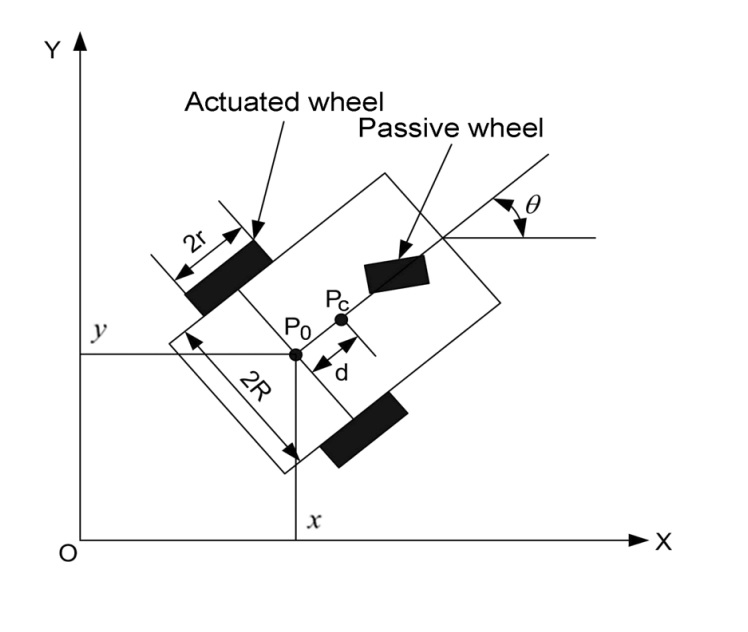
\includegraphics[width=8cm]{img/MobileRobot.jpg}
	\شرح{مدل پایه مورد بررسی \مرجع{park2009simple}}
	\برچسب{ربات}
\end{figure}
مدل کلی این ربات به سه زیر بخش سینماتیک،‌ دینامیک خارجی و دینامیک داخلی عملگر تقسیم می‌شود که متغیر های حالت مربوط به هر بخش به ترتیب به صورت
$
q=
\begin{bmatrix}
	x  & y & \theta
\end{bmatrix}^T 
\in \mathbb{R}^3
$
،
$
z=
\begin{bmatrix}
	v_1  & v_2
\end{bmatrix}^T 
\in \mathbb{R}^2
$
و
$
i_a=
\begin{bmatrix}
	{i_a}_1  & {i_a}_2 
\end{bmatrix}^T 
\in \mathbb{R}^2
$
می‌باشد که در آن ها 
$x$
،
$y$
و
$\theta$
به ترتیب طول و عرض نقطه \مل{P}
و $\theta$ زاویه ربات، 
$v_1$
و
$v_2$
سرعت چرخ های عقب و 
${i_a}_{1}$
و
${i_a}_{2}$
جریان دو موتور می‌باشد.
روابط مربوط به بخش سینماتیک و دینامیک خارجی به فرم زیر خواهد بود \مرجع{do2004simultaneous}:
\begin{equation}
	\dot{q}=J(q)z = 0.5r
	\begin{bmatrix}
		\cos\theta & \cos\theta \\
		\sin\theta & \sin\theta   \\
		R^{-1}       & -R^{-1}
	\end{bmatrix}
	\begin{bmatrix}
		v_1  \\
		v_2
	\end{bmatrix}
\end{equation}
\begin{equation}
	\tau=M\dot{z} + C(\dot{q})z + Dz + \tau_d
\end{equation}
که در آن:
\begin{equation*}
	M = 
	\begin{bmatrix}
		m_{11} & m_{12} \\
		m_{12} & m_{11} 
	\end{bmatrix}
\end{equation*}
\begin{equation*}
	m_{11} = 0.25R^{-2}r^2(mR^2 +I)+I_w
\end{equation*}
\begin{equation*}
	m_{12} = 0.25R^{-2}r^2(mR^2 -I)
\end{equation*}
\begin{equation*}
	m = m_c + 2m_w
\end{equation*}
\begin{equation*}
	I = m_c d^2 +2m_w R^2 +I_c +2 I_m
\end{equation*}
\begin{equation*}
	C(\dot{q}) = 0.5 R^{-1}r^2m_cd
	\begin{bmatrix}
		0 & \dot{\theta} \\
		\dot{\theta} & 0 
	\end{bmatrix}
\end{equation*}
\begin{equation*}
	D = 
	\begin{bmatrix}
		d_{11} & 0\\
		0 & d_{22} 
	\end{bmatrix}
\end{equation*}
\begin{equation*}
	\tau =
	\begin{bmatrix}
		\tau_1 & \tau_2  
	\end{bmatrix}^T 
\end{equation*}
\begin{equation*}
	\tau =
	\begin{bmatrix}
		{\tau_d}_1 & {\tau_d}_2  
	\end{bmatrix}^T 
\end{equation*}
در این روابط،
$
m_c
$
و
$
m_w
$
به ترتیب جرم بدنه ربات و جرم چرخ ها؛
$
I_c
$
،
$
I_w
$
و
$
I_m
$
به ترتیب ممان اینرسی بدنه ربات نسبت به محور عمودی گذرنده از نقطه \مل{P0}،
ممان اینرسی چرخ به همراه موتور حول محور چرخ و ممان اینرسی چرخ و موتور حول قطر؛ 
$d_{11}$
،
$d_{22}$
ضرایب دمپینگ؛
$
\tau \in \mathbb{R}^2
$
بردار گشتاور کنترلی اعمال شده به چرخ ها و
$
{\tau}_d \in \mathbb{R}^2
$
بردار اغتشاشات شامل دینامیک مدل نشده می‌باشند.\\
روابط مربوط به دینامیک داخلی عملگر نیز به فرم زیر خواهد بود \مرجع{das2006design}:
\begin{equation}
	\begin{cases}
		\tau_m = K_T i_a \\
		u = R_ai_a +L_a \dot{i_a} +K_E \dot{\theta_m}
	\end{cases}
\end{equation} 
که در آن 
$
\tau_m = 
\begin{bmatrix}
	{\r_m}_1 & {\r_m}_2  
\end{bmatrix}^T 
$
گشتاور تولید شده توسط موتور \مل{DC}؛
$
K_T = diag
\begin{bmatrix}
	{K_t}_2 & {K_t}_2  
\end{bmatrix}
$
ثوابت گشتاور موتور؛
$
i_a \in \mathbb{R}^2
$
جریان؛
$
R_a= diag
\begin{bmatrix}
	{r_a}_1 & {r_a}_2  
\end{bmatrix}
$
مقاومت؛ 
$
L_a= diag
\begin{bmatrix}
	{l_a}_1 & {l_a}_2  
\end{bmatrix}
$
ضرایب خودالقایی؛
$
K_E = diag
\begin{bmatrix}
	{K_e}_1 & {K_e}_2  
\end{bmatrix}
$
ثابت نیروی ضد محرکه و
$
\dot{\theta}_m =
\begin{bmatrix}
	{\dot{\theta}}_1 & {\dot{\theta}}_2  
\end{bmatrix}
$
سرعت زاویه ای موتور می‌باشند. \\
روابط  موتور و ربات نیز با استفاده از رابطه نسبت چرخ دنده ها به هم مربوط می‌شود:
\begin{equation}
	\begin{cases}
		\tau = N K_T i_a \\
		u = R_ai_a +L_a \dot{i_a} + NK_E \dot{\theta_m}
	\end{cases}
\end{equation} 
که در آن 
$
N = 
diag 
\begin{bmatrix}
	n_1 & n_2  
\end{bmatrix}
$
نسبت چرخ دنده ها می‌باشد.\\
بنابراین به طور خلاصه با تعاریف 
$
x_1 = q
$
،
$
x_2 = z
$
و
$
x_3 = i_a
$
روابط این بخش به طور خلاصه به صورت زیر بیان می‌شود:
\begin{equation}
	\dot{x}_1= J(x_1)x_2
\end{equation}
\begin{equation}
	\dot{x}_2= M^{-1}(-C(\dot{x}_1)x_2 - Dx_2 -\tau_d +NK_T x_3)
\end{equation}
\begin{equation}
	\dot{x}_3= {L_a}^{-1}(u-R_ax_3-NK_Ex_2)
\end{equation}
\زیرقسمت{طراحی کنترل کننده}
\ورودی{controler-design}
\قسمت{مقاله \ب}
\ورودی{Cheein}
\زیرقسمت{مقاله \پ}
\ورودی{shojaei}